\documentclass{rapport_gls}

\begin{document}

\begin{titlepage}
\begin{center}

% Titre
   \textsc{\Large ENSEEIHT : Génie du Logiciel et des Systèmes (GLS)}\\[6cm]
\textsc{\large Rapport de projet}\\
\HRule \\
\huge{GLS : Rapport de projet\\}
\HRule \\[3cm]

\includegraphics[height=4cm]{../Images/gears.pdf}
\vfill

\LARGE{Matthieu Pizenberg}\\[1em]
\large{\today}

\end{center}
\end{titlepage}


\newpage

\tableofcontents

\newpage

\chapter{Les métamodèles SimplePDL et PetriNet}
Pour l'ensemble de la chaine de transformation on aura besoin des métamodèles SimplePDL et PetriNet, on définit donc ces deux métamodèles ainsi que des exemples de modèles qui serviront à faire les tests.

\section{SimplePDL}
On a ajouté au modèle SimplePDL la gestion des ressources.
Pour celà, on a introduit :
\begin{itemize}
\item Ressource : une ressource ayant un nom et étant présente en une certaine quantité
\item Need : un besoin représentant un nombre de ressources d'un certain type
\item NeedSet : un ensemble de besoins nécessaires à la réalisation d'une WD
\end{itemize}

\vspace{1em}
Voilà un diagramme représentant le métamodèle SimplePdl que j'ai utilisé :
\begin{center}
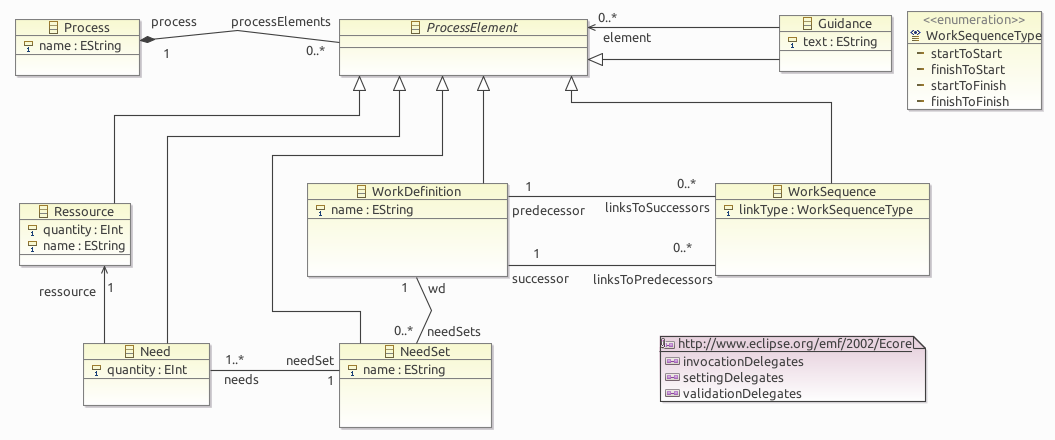
\includegraphics[width=\textwidth]{../Images/model_pdl.png}
\end{center}

\newpage
\section{PetriNet}
\newpage
\begin{center}
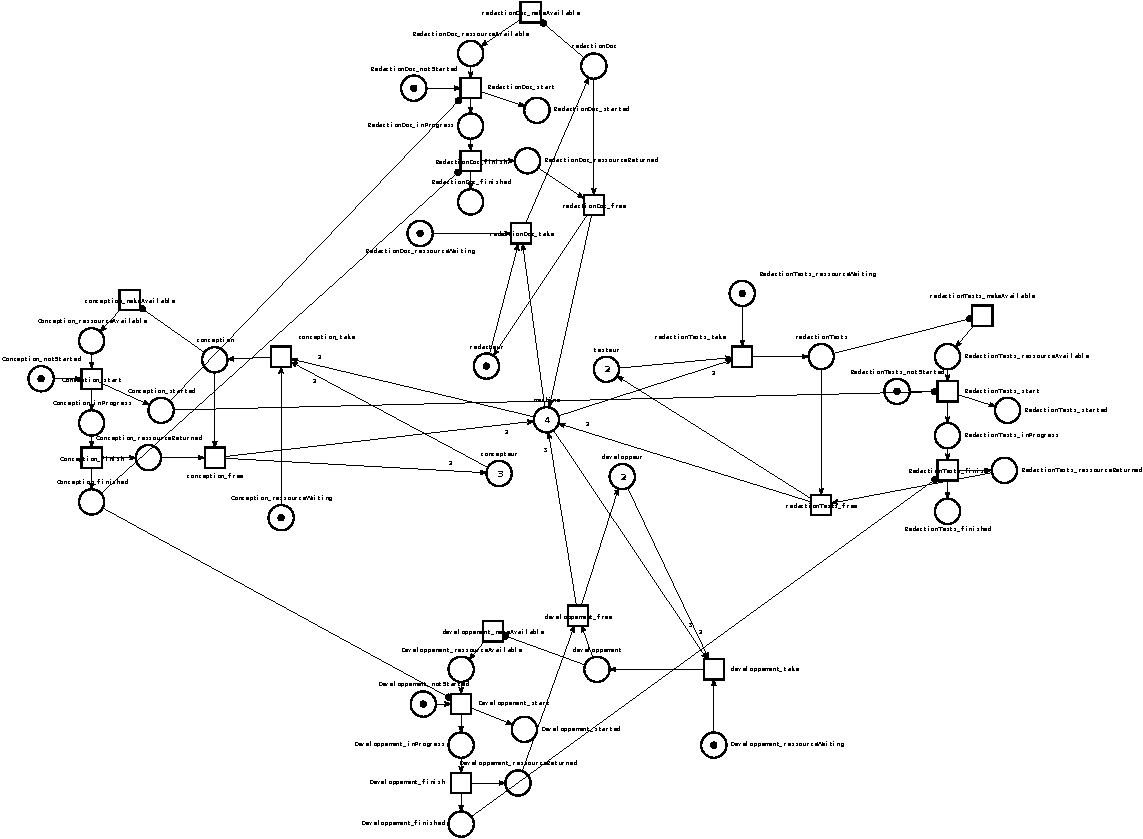
\includegraphics[width=1\textwidth]{../Images/processus_net.pdf}
\end{center}

\newpage
\section{Exemples de modèles}
Voici quelques exemples de modèles SimplePDL (sans ressources) :

\begin{figure}[h]
   \centering
   \subfloat[Processus simple]{\label{process_simple_pdl}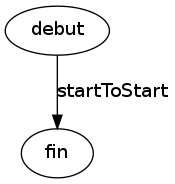
\includegraphics[width=0.18\textwidth]{../Images/model_process_simple_pdl.png}}
   \subfloat[Processus]{\label{process_pdl}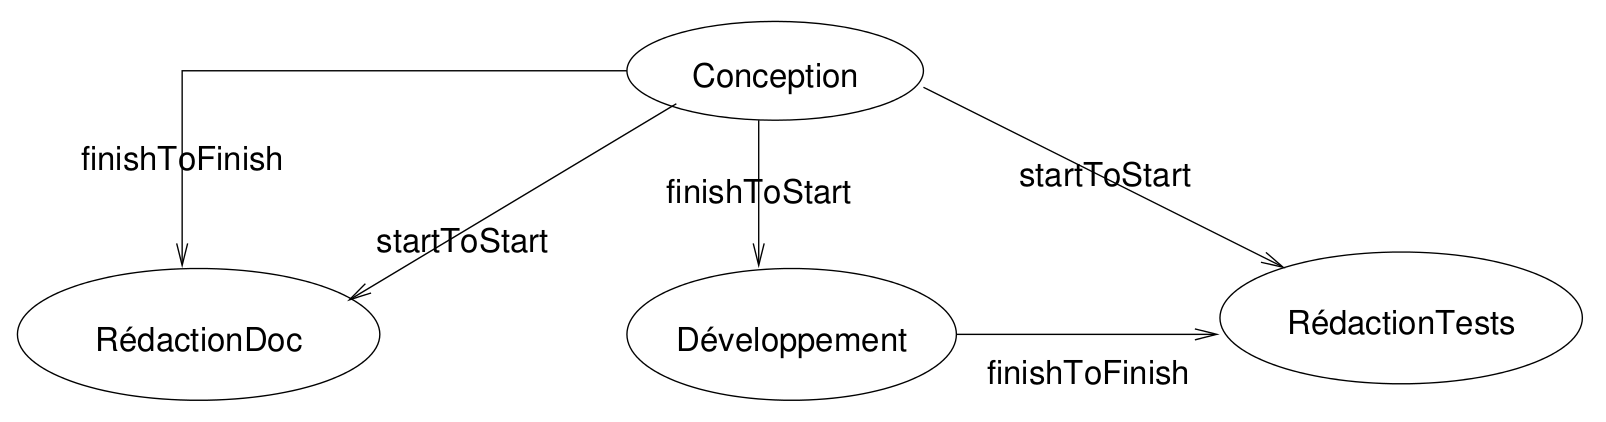
\includegraphics[width=0.7\textwidth]{../Images/model_process_pdl.png}}
   \caption{Exemples de modèles de processus SimplePDL}
\end{figure}

\vspace{1em}
Et quelques exemples de modèles PetriNet :
\begin{figure}[h]
   \centering
   \subfloat[Exemple]{\label{exemple_net}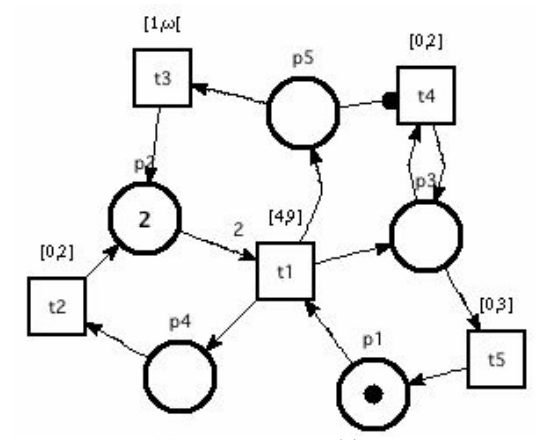
\includegraphics[width=0.5\textwidth]{../Images/model_exemple_net.png}}
   \subfloat[4 saisons]{\label{saisons_net}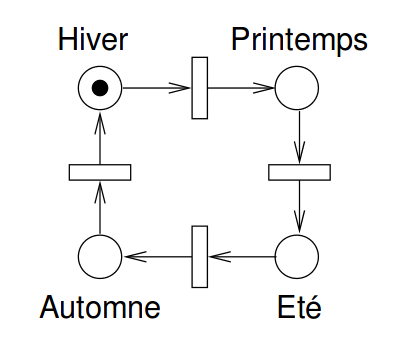
\includegraphics[width=0.5\textwidth]{../Images/model_saisons_net.png}}
   \caption{Exemples de modèles de réseaux de pétri}
\end{figure}


\chapter{Transformations modèle à modèle (M2M)}
Pour analyser les modèles de processus en SimplePDL, on va avoir besoin de les transformer en réseaux de pétri.
Pour çà, on doit effectuer des transformations ModelToModel (M2M) avec comme origine un modèle SimplePDL et comme arrivée un modèle PetriNet.\\

On utilise l'outil ATL (plugin pour Eclipse) afin d'effectuer ces transformations.

\section{L'outil ATL}
On montre ici brièvement la syntaxe d'un fichier ATL avec quelques exemples :

\lstset{
   language={}
}
\begin{lstlisting}
-- Traduire un Process en un PetriNet de même nom
rule Process2PetriNet {
   from p: simplepdl!Process
   to pn: petrinet!PetriNet (name <- p.name)
}
\end{lstlisting}

Les règles de transformation sont exprimées avec le mot-clé "rule".
Les mots "from" et "to" permettent d'identifier les éléments de la transformation.


\begin{lstlisting}
-- Traduire une WorkSequence en un motif sur le réseau de Petri
rule WorkSequence2PetriNet {
   from ws: simplepdl!WorkSequence
   to
      a_ws: petrinet!Arc(
         petriNet <- ws.getProcess(),
         readOnly <- true,
         multiplicity <- 1,
         predecessor <- thisModule.resolveTemp(ws.predecessor,
            if((ws.linkType = #finishToStart) or (ws.linkType = #finishToFinish))
               then 'p_finished'
               else 'p_started'
            endif),
         successor <- thisModule.resolveTemp(ws.successor,
            if((ws.linkType = #finishToStart) or (ws.linkType = #startToStart))
               then 't_start'
               else 't_finish'
            endif)
         )
}
\end{lstlisting}

La commande "resolveTemp" permet d'identifier un élément parmi ceux présents dans les règles de transformations.

\section{De SimplePDL à PetriNet}
Le code de transformation complet étant assez long je vais ici expliquer à l'aide de graphiques les opérations pour transformer les éléments SimplePDL en éléments de réseau de pétri :\\

\subsection{WorkDefinition WD}
J'ai voulu modifier au minimum la structure des WD et des WS dont on avait les transformations avant l'ajout des ressources aux modèles.
Ainsi on assure une évolution simple des WD et WS.\\

On commence par une WorkDefinition WD. Avec les ressources en plus, une WD a besoin de savoir si des ressources sont disponibles pour pouvoir démarrer une activité.
\begin{itemize}
   \item On ajoute donc une place ressources\_available reliée à la transition start d'une WD.
   \item On ajoute également une place ressources\_wait (marquée à 1) pour indiquer que la WD est en attente de ressources
   \item Enfin on ajoute une place ressources\_returned reliée en sortie de la transition finish qui inque que la WD a fini d'utiliser les ressources
\end{itemize}

\vspace{1em}
On a donc ajouté 3 places et 2 arcs à notre WD. Voici un graphique récapitulatif :

\begin{figure}[h]
\centering
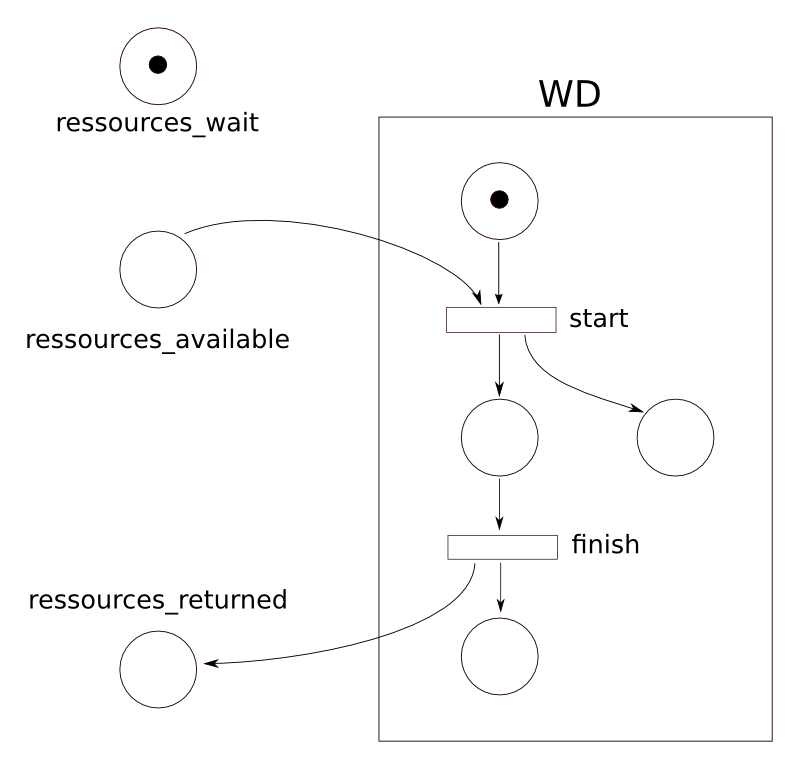
\includegraphics[width=0.6\textwidth]{../Images/WD2petri.png}
\label{WD2petri}
\caption{Transformation d'une WorkDefinition WD en réseau de pétri}
\end{figure}

\newpage
\subsection{NeedSet}
Je ne décris pas le besoins (Need) car il s'agit d'une simple place avec un marquage correspondant à "quantity".\\

Chaque ensemble de besoins (NeedSet) correspond à un ensemble constitué de :
\begin{itemize}
   \item une place "set" pour indiquer de quel NeedSet il s'agit
   \item 3 transition :
      \begin{itemize}
         \item "take" qui est reliée à chaque ressource nécessaire pour le NeedSet
         \item "makeAvailable" entre la place "set" du NeedSet et la place "ressources\_available" de la WD
         \item "return" reliée aux ressources qui vont être rendues
      \end{itemize}
   \item enfin les arcs qui vont bien (voir schéma)
\end{itemize}

\begin{figure}[h]
\centering
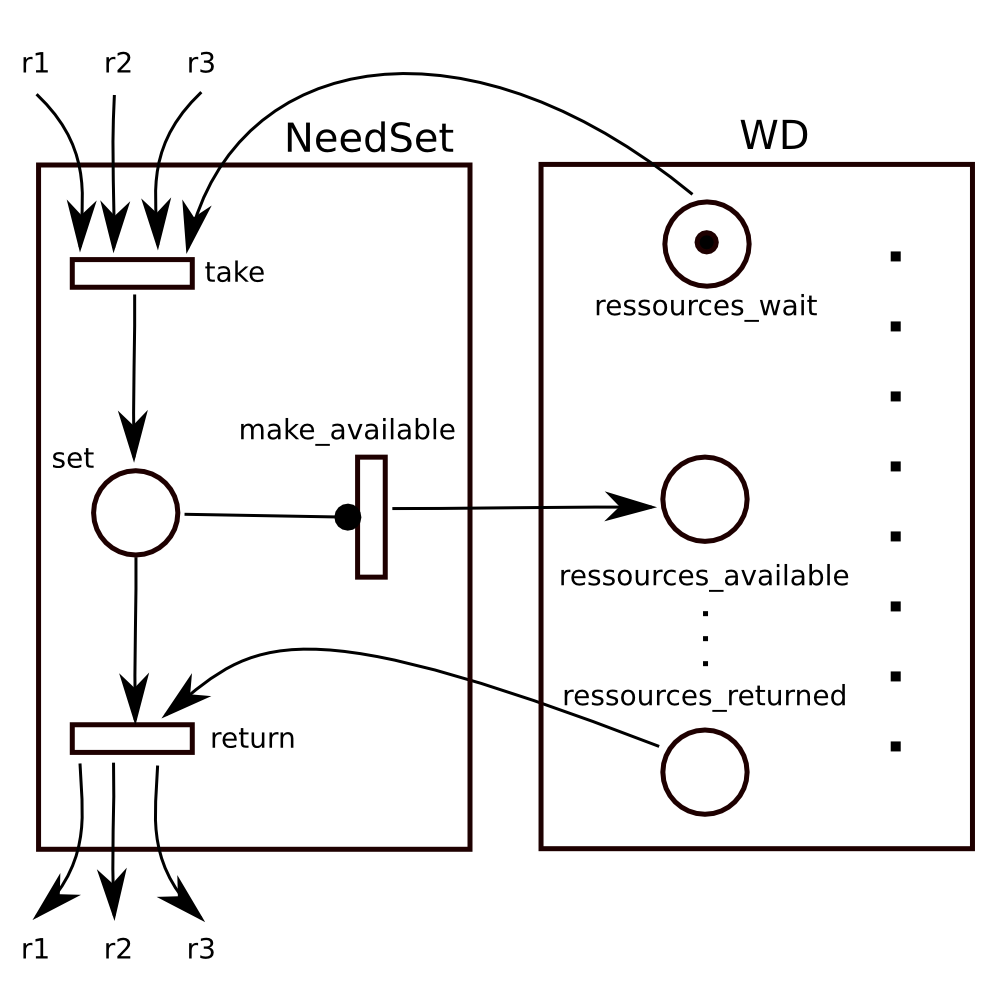
\includegraphics[width=0.6\textwidth]{../Images/NeedSet2petri.png}
\label{WD2petri}
\caption{Transformation d'un ensemble de besoins NeedSet en réseau de pétri}
\end{figure}



\chapter{Transformations modèles à textes (M2T)}
Les transformations M2T (ModelToText) permettent d'obtenir des fichiers avec uns syntaxe respectant certaines contraintes.
Un unique modèle peut être représenté par différents fichiers ayant des syntaxes différentes, facilitant ainsi l'usage dans un environnement donné.\\

Pour effectuer ces transformations nous avons utilisé Acceleo, lui ausi intégré à Eclipse sous la forme d'un plugin.

\section{L'outil Acceleo}
Le langage utilisé par Acceleo (d'extension .mtl) est un langage de template.
On construit bout par bout notre fichier texte à l'aide de boucles, de conditions et de requêtes.\\

Voilà un exemple de boucle avec condition :
\lstset{
   language={}
}
\begin{lstlisting}
[for (pl : Place | petriNet.petriNetElements->getPlaces())]
[if (pl.marking > 0)]pl [pl.name/] ([pl.marking/])[/if]
[/for]
\end{lstlisting}

Et voilà un exemple de requête pour récupérer les places d'un réseau de pétri :
\begin{lstlisting}
[query public getPlaces(elements : OrderedSet(PetriNetElement)) : OrderedSet(Place) = 
   elements->select( e | e.oclIsTypeOf(Place) )
      ->collect( e | e.oclAsType(Place) )
      ->select( e | e.marking > 0 )
      ->asOrderedSet()
/]
\end{lstlisting}


\newpage
\section{PetriNet}
\newpage
\begin{center}
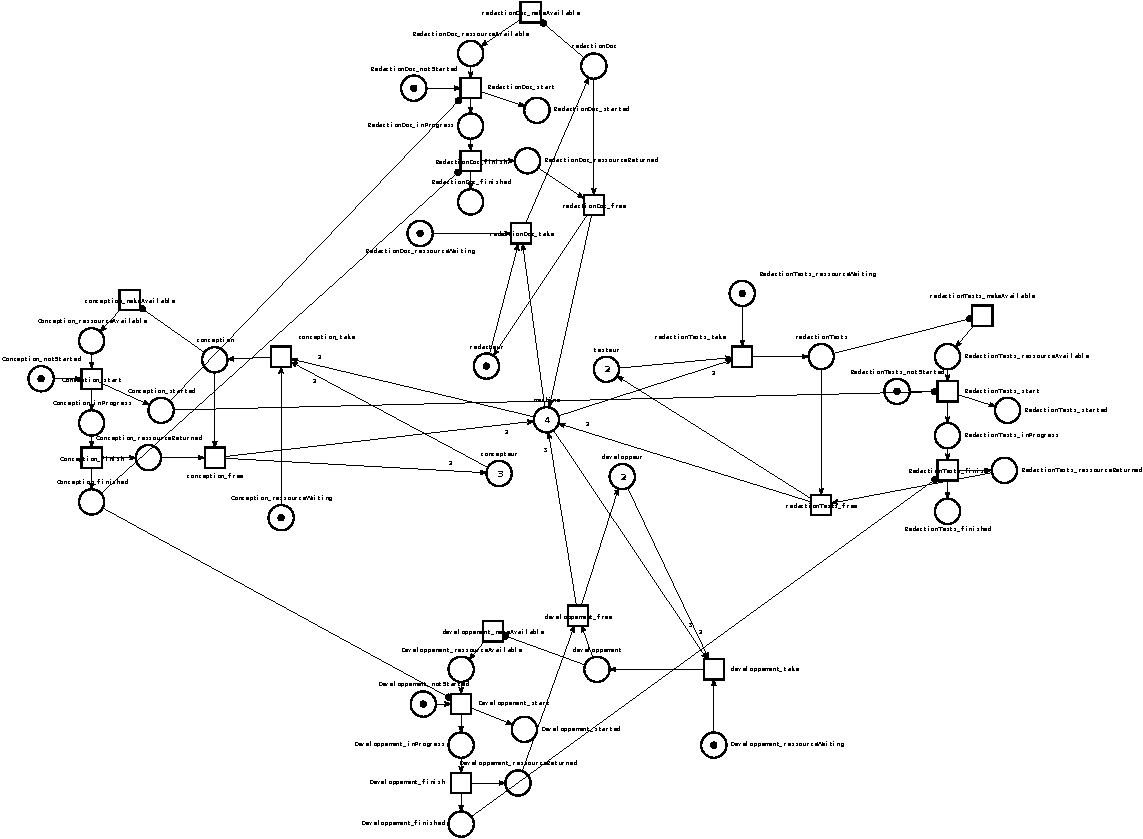
\includegraphics[width=1\textwidth]{../Images/processus_net.pdf}
\end{center}


\chapter{Transformations textes à modèles (T2M)}
Enfin nous avons besoin de pouvoir saisir rapidement et simplement des modèles de réseau de pétri ou SimplePDL.
Pour celà, on utilise la transformation T2M (TextToModel) qui permet d'établir une syntaxe pour un modèle.
L'outil que l'on utilise est également intégré à Eclipse sous la forme d'un plugin, il s'agit d'Xtext.

\section{L'outil Xtext pour SimplePDL et PetriNet}
Xtext permet de spécifier la syntaxe d'un fichier décrivant un modèle.
Cette spécification permet également la construction automatique du métamodèle correspondant à la syntaxe concrète décrite.\\

En fait, il apparait que le métamodèle construit est légèrement différents du métamodèle initial.
Ceci est d'autant plus vrai que la syntaxe est simplifiée et s'éloigne de la structure du modèle.
Ce n'est pas si grave, puisque l'on connait maintenant les outils permettant de faire des transformations M2M.\\

Voilà à quoi ressemble la syntaxe d'un fichier xtext, ici le contenu du xtext pour petrinet :

\lstset{
   language={}
}
\begin{lstlisting}
PetriNet :
   'petrinet' name=ID '{'
      petriNetElements+=PetriNetElement*
   '}'
   ;

PetriNetElement :
   Node
   | Arc
   ;

Node :
   Place
   | Transition
   ;

Place :
   'place' name=ID ('('marking=INT')')?
   ;

Transition :
   'transition' name=ID
   ;

Arc :
   'arc' ('('multiplicity=INT')')? (readOnly ?= 'r')?
   'from' predecessor=[Node]
   'to' successor=[Node]
   ;
\end{lstlisting}

Le fichier xtext pour notre syntaxe pdlx (pdl extended for ressources) est donnée dans les sources.\\

On donne ici un exemple en .pdlx :

\begin{lstlisting}
process test {
   wd conception
   wd redactionDoc
   wd developpement
   wd redactionTests

   ws s2s from conception to redactionDoc
   ws f2f from conception to redactionDoc
   ws f2s from conception to developpement
   ws s2s from conception to redactionTests
   ws f2f from developpement to redactionTests

   r concepteur (3)
   r developpeur (2)
   r machine (4)
   r redacteur (1)
   r testeur (2)

   set set_conception wd conception
      n concepteur(2) set set_conception
      n machine(2) set set_conception
   set set_redactionDoc wd redactionDoc
      n machine(1) set set_redactionDoc
      n redacteur(1) set set_redactionDoc
   set set_developpement wd developpement
      n developpeur(2) set set_developpement
      n machine(3) set set_developpement
   set set_redactionTests wd redactionTests
      n testeur(2) set set_redactionTests
      n machine(2) set set_redactionTests
}
\end{lstlisting}

Et pour un fichier en .petri :

\begin{lstlisting}
petrinet petrinet1 {
   place place1
   place place2 (2)
   transition transition1
   arc r from place1 to transition1
   arc (2) from transition1 to place2
}
\end{lstlisting}


\chapter{Conclusion}
On a presque complété toute la chaine de transformation des modèles.
Par manque de temps, je n'ai pas fait la partie concernant la vérification de modèle.\\

Ce projet m'a beaucoup intéressé, mais il semble qu'il manque un élément dans la chaine de transformation : La génération d'un modèle en .xmi à partir d'un modèle respectant la syntaxe établie avec Xtext.
Ceci permettrait de rendre vraiment efficace la génération de modèle.


\end{document}
